%!TEX root = ../template.tex
%%%%%%%%%%%%%%%%%%%%%%%%%%%%%%%%%%%%%%%%%%%%%%%%%%%%%%%%%%%%%%%%%%%%
%% chapter4.tex
%% NOVA thesis document file
%%
%% Chapter with lots of dummy text
%%%%%%%%%%%%%%%%%%%%%%%%%%%%%%%%%%%%%%%%%%%%%%%%%%%%%%%%%%%%%%%%%%%%
\chapter{State of the Art}
\label{cha:SotA}


\section{Social Networks}
\label{sec:SocialNet}

%Beggining of Social Network Analysis
\par
Social Network Theory and Analysis, these are the area that study the currently emerging networks. \\
Network communication can be found all around us human bodies have them (Neves et al, 2008), physics, politics, computer science, etc. Socially, in later years, networks have been developed used many important websites like facebook, twitter, Instagram. This has created a new importunity for marketing and analysis. 
Since this work is mainly focused on feedback I’ll focus more on that particular area.
%Create Node Image Showing a Centralized network, Decentralized and Distributed

\begin{figure}[htbp]
	\centering
	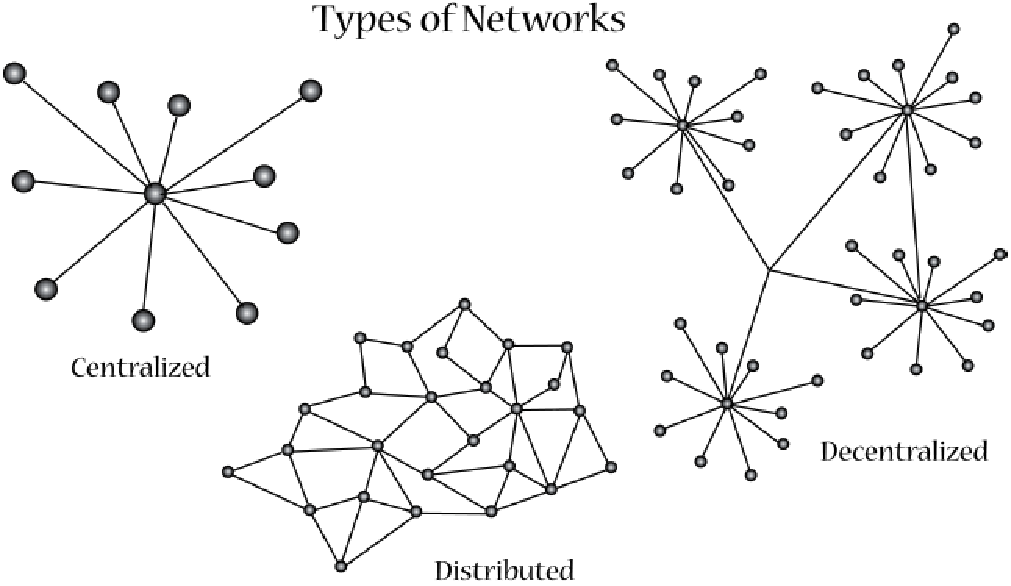
\includegraphics[height=2in]{network-types-pdf}
	\caption{Network Types}
	\label{fig:NetworkTypesImg}
\end{figure}

Figure \ref{fig:NetworkTypesImg} shows some examples of network diagrams. Centralized networks are highly advantageous  connection wise, everyone can give information to each other within 2 step, but fail when the centralized node is offline for some reason, this stops the entire network.
\par
Before internet, companies had to rely on Decentralized networks to gather feedback, some still do. By decentralizing, the amount of nodes that fail when the upper node disappear is lower, although it still happens. The big advantage of this layout is that it can easily become a Distributed network. Outer and lower connection nodes can easily connect to each other and create redundancy. 
\begin{figure}[htbp]
	\centering
	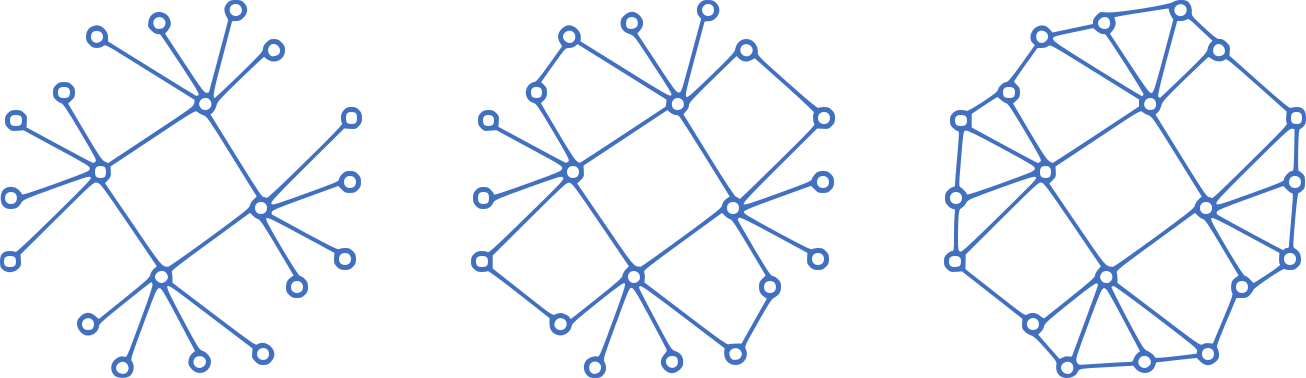
\includegraphics[width=\textwidth]{Decent-Distri-pdf}
	\caption{Decentralized to Distributed}
	\label{fig:Decent-Distri}
\end{figure}

\par
Distributed networks, occur when all nodes are connected to the same amount of nodes Figure \ref{fig:Decent-Distri}. This means that everyone has the same importance in the network. a layout like this is extremely utopic when thinking about feedback analysis. 
\par
While everyone has their own, valid, opinion on a product, people like celebrities can spread their opinion faster than a kinder gardener. Realistically, decentralized networks are the most common occurrence.

%End of Social Network Analysis

%\lipsum[1-100]
%\lipsum[1-100]
%\lipsum[1-100]
% \lipsum[1-100]
% \lipsum[1-700]
% \lipsum[1-700]
% \lipsum[1-700]
% \lipsum[1-700]
% \lipsum[1-700]
% \lipsum[1-700]
% \lipsum[1-700]
% \lipsum[1-700]
